\documentclass{article}

% if you need to pass options to natbib, use, e.g.:
\PassOptionsToPackage{numbers, compress}{natbib}
% before loading neurips_2018

% ready for submission
% \usepackage{neurips_2018}

% to compile a preprint version, e.g., for submission to arXiv, add add the
% [preprint] option:
%     \usepackage[preprint]{neurips_2018}

% to compile a camera-ready version, add the [final] option, e.g.:
     \usepackage[final]{neurips_2018}

% to avoid loading the natbib package, add option nonatbib:
%     \usepackage[nonatbib]{neurips_2018}

\usepackage[utf8]{inputenc} % allow utf-8 input
\usepackage[T1]{fontenc}    % use 8-bit T1 fonts
\usepackage{hyperref}       % hyperlinks
\usepackage{url}            % simple URL typesetting
\usepackage{booktabs}       % professional-quality tables
\usepackage{amsfonts}       % blackboard math symbols
\usepackage{nicefrac}       % compact symbols for 1/2, etc.
\usepackage{microtype}      % microtypography
\usepackage{multirow}       % table building
\usepackage{graphicx}       % including images
\usepackage[english]{babel}
\usepackage[shortlabels]{enumitem} % enumerating
\usepackage{subfigure}       % subfigures

% \usepackage[square,numbers]{natbib}
\bibliographystyle{abbrvnat}

\graphicspath{ {./media/} }

\title{Combined GCN LSTM for vertex classification}

% The \author macro works with any number of authors. There are two commands
% used to separate the names and addresses of multiple authors: \And and \AND.
%
% Using \And between authors leaves it to LaTeX to determine where to break the
% lines. Using \AND forces a line break at that point. So, if LaTeX puts 3 of 4
% authors names on the first line, and the last on the second line, try using
% \AND instead of \And before the third author name.

\author{
Idan   ~Ben-Ami\\
  Department of Computer Science\\
Bar Ilan  University\\
Ramat Gan, Israel, 5290000 \\
  \texttt{idanbena@gmail.com} \\
\And
  Yoram  ~ Louzoun\\
  Department of Mathematics\\
Bar Ilan  University\\
Ramat Gan, Israel, 5290000 \\
  \texttt{louzouy@math.biu.ac.il} \\
 }

\begin{document}
% \nipsfinalcopy is no longer used

\maketitle

\begin{abstract}
Graph Convolutional Networks (GCN) have emerged as one of the best methods to classify nodes using either external information or the graph structure itself through label propagation. However, current GCN approaches are based on a single snapshot of a graph or multi-graphs. We propose to combine GCN with recurrent neural networks and show that such a formalism outperforms the precision obtained in single graph-based predictions. We tested this method on a dataset of firms product similarity and shown it can be used to predict the future success of companies or forthcoming collapse. A similar comparison on a blog network and a prediction of the activity of bloggers produces similar results.

\end{abstract}
\section{Introduction and previous research}

One of the central assumptions in node classification tasks is that neighboring nodes have similar classes. This has been extensively used in node classification tasks, and in machine learning based approaches to predict node classes. Such approaches are now often denoted as graph machine learning or graph neural networks (i.e. machine learning where the input is a graph/network, in contrast with neural network, where the network topology is not directly related to the observations). Three main approaches have been proposed to take advantage of a graph in machine learning:

\begin{itemize}
\item   Regularization of the output requiring that neighboring nodes should have similar classes, and graph partitioning. Such methods often include partitioning the graphs based on the eigenvalues of the Laplacian or weighted Laplacian \cite{dhillon2007weighted,karypis1995analysis}. Other works have used variants of this idea, each using smoothness and graph distance (e.g.,\cite{belkin2004semi,sindhwani2005linear}). An alternative approach is to use quadratic penalty on the difference between neighboring nodes \cite{zhou2004learning,zhu2003semi}.
\item   Graph-based label propagation. Multiple diffusion and information propagation models have been proposed \cite{rosenfeld2017semi}. For example, DeepWalk \cite{perozzi2014deepwalk}, where a truncated random walk is performed on nodes and used to project nodes to a multidimensional real space. Planetoid \cite{yang2016revisiting} also uses random walks combined with negative sampling. Duvenaud et al. used a translation of subgraphs to hash functions for a similar task in the context of molecule classifications \cite{duvenaud2015convolutional}. A very similar approach was presented by Leskovech by projecting nodes minimizing the distance of neighbored nodes in a truncated random walk (Node2vec \cite{grover2016node2vec}). The DNGR model \cite{cao2016deep} uses random walk to compute the mutual information between points A Multi-Dimensional-Scaling (MDS) projection of the points in the graphs was also used for a similar goal \cite{belkin2002laplacian,levy2015improving}. An alternative approach was inspired by word embedding methods \cite{mikolov2013distributed} such as word2vec. These methods use the graph to define a “context” in relation to which the node embedding is constructed. When the data includes only the graph, the embeddings are used as features and fed into existing predictors \cite{perozzi2014deepwalk}. When the data includes node features, these embeddings are used as an additional regularization term to a standard loss over the labeled nodes \cite{yang2016revisiting}. Refex \cite{henderson2011s} defines local features to translate each node to a vector features and use those to predict classes.
\item   Graph Convolution Networks (GCN) to learn the relation between the input of a node and its neighbors to its class. Recently, Kipfs and collaborators, in a seminal work, proposed a simplification of spectral based convolutions \cite{kipf2016semi,schlichtkrull2018modeling}, and instead use a two-layer approach, where the weights of each layer are multiplied by a derivative of the adjacency matrix. They tested their work on multiple graphs with labeled nodes including CiteSeer, Cora Pubmed and Nell. GCN approaches can also be used where the graph is used as a filter on the input. Most such convolutions are spectral (use the Laplacian eigenvectors). However, recent methods are based on random filters \cite{atwood2016diffusion,bruna2013spectral,henaff2015deep}. Similar formalisms were used to study not only single snapshots but also time series of graphs, mainly in image analysis \cite{seo2018structured}.

\end{itemize}

These methods presume a single graph or a single multi-graphs and static node classifications. However, in many realistic scenarios, both the graph and the labels evolve. An interesting example would be companies labeled as successful or not, and graphs representing the relation between such companies. We here analyze a company similarity network over 17 years and show that a combination of GCN with LSTM can improve the accuracy of the prediction of success and bankruptcies.

\section{Main contributions of current research}
The main advances presented here compared with existing methods are:
\begin{itemize}
\item   Using topological information or the sum of first and second neighbors in each class of the training set as input to GCN in absence of external information.
\item   Combination of directed label propagation, topology and external information in one coherent framework.
\item   Combination of this framework into a recurrent network formalism to handle evolving graphs, and showing it outperforms static approaches. 
\end{itemize}

\section{Model and data description}
Our main goal is to predict whether companies would collapse next year using both ranking information and a network similarity product. Jing Fang et al \cite{fan2018combined} introduced this network and the task, and we follow them by integrating their task into a GCN formalism for each year, and testing whether combing GCNs from multiple years under one combined LSTM outperforms a GCN for each time point (TP).

The advantage of such a formalism is the possibility of using information from previous years to improve the accuracy of the prediction this year. Another advantage is the production of a single GCN for all years leading to a simpler interpretation of the results. We show here that the proposed approach does improve the average accuracy. 

Formally our model is as follows, Given a set of TP: $TP=1 \to k$ and for each time point we are given an undirected graph represented by an adjacency matrix $A^k$, a label for each node $i$ in the graph $z_{k}(i)$ and possibly some external input on each node $\vec{x}_{k}(i)$. We use a GCN $H^k$ to classify the labels using either only the graph topology or a combination of the graph topology and the external input. We then tested multiple methods to represent the graph topology and computed the resulting accuracy. We then test whether using the GCN output as the input to a LSTM and learning the labels using the LSTM produces a higher accuracy. We tested 4 configurations:
\begin{itemize}
\item   Pure GCN model on each year – yielding $n$ models - one for each snapshot (year) to predict the outcome in the following snapshot (i.e. prediction from the interactions in year $k$ the collapse of the company in year $k+1$).
\item   Pure GCN model trained on all years simultaneously – yielding a single model, compatible for all snapshots (i.e. shared weights between the GCN of all years). This model was trained in each TP. Thus at each TP, we recompute the model over all previous TP.
\item   Two phases models, where we first train the single model learned (as above), and then we use it’s one before the last layer as the input to an RNN.
\item   A combined model where the combined GCN and RNN are trained simultaneously.
\end{itemize}

\subsection {Different static model for each year}
We extended the GCN model developed by Thomas Kipf et al. \cite{kipf2016semi}. Each GCN layer is defined as: $$X_{n+1}=\sigma(A*X_{n}*W_n)$$ where $A$ is the adjacency matrix, $X$ is the input from the previous layer, and $W$ are the weights of the current layer. The activation function for intermediate layers was the ReLu function, and the last layer was linear. Dropout rates of 40\% and $L2$ regularization with a weight of 0.001 were used. The models were trained for 200 epochs with a Negative-Log-Likelihood loss on a weighted distribution of classes (to correct the imbalanced distribution of labels) and an Adam optimizer. The GCN had three internal layers of sizes 100 and 35 and 20 in all models studied. The main difference between the current model and existing GCN is the usage of a topology or neighbors' tags as input to the nodes. In the absence of any external information on the nodes, we propose to use one of the two possible inputs: A) Characterize each node by a vector of topological attributes, and use this vector as an input, B) Compute the number of neighbors and second neighbors that have a given tag and use this number as the input layer of the GCN. This creates a vector of twice the number of possible tags for each node. When external information is available we introduce the external information and topological

%The extension comes through the incorporation of an asymmetric adjacency matrix. In this model we do not lose the direction of the graph, which contains topological information. We incorporate the direction by taking the adjacency matrix (asymmetric in directed graph) and concatenate its transpose to it – creating a$ 2n x n$ adjacency matrix. The dimension of the output of each layer is: $[(2NxN)*(Nxi_n )*(i_n xo_n )]=2Nxo_n$., which in turn is passed to the next layer following a rearrangement of the output by splitting and concatenating it to change dimensions from  - $2NxO_n$  to $ Nx2O_n$. 

%At first, we wanted to asses our data on the base model (MultiLayerGCN and CombinedGCN). In this stage, we performed complete learning of the base model on each of the snapshots, independently of each other. Both these base models support directed graphs and undirected graphs using a symmetric or an asymmetric version correspondingly.

\subsection{Combined static model for all the years}
We used the two basic models above (with and without external information) and trained each of them on all snapshots simultaneously. Unlike the previous stage, the process yields unified models that are learned and tested over all the snapshots together. So, the only difference between this approach and the previous is weight sharing between the $TP$. The models were again trained for 200 epochs with a Negative-Log-Likelihood loss on a weighted distribution of classes and an Adam optimizer. In both approaches (shared and distinct weights), the only parameter that was varied was the $L2$ regularization and values between $1.e-4$ and $1.e-1$ were tested in $log10$ jumps of 1 log. All results are presented as the average of 3 runs, and the resulting standard error.

\subsection{ Two-phase model – with separate GCN and RNN}
In this model, the GCN was combined with an RNN that handles the network dynamics. First, we trained the unified model for all the years as above. This unified model still represents a static approach for the classification. We then trained the RNN. The input for the RNN layer was the one before the last layer of the static model. To do so, we forward propagated each TP through the static part of the model, so that the input of the second phase is of dimensions $[N_{seq}xN_{nodes}*O_{l-1}]$ where $N_{seq}=17$ – the sequence length (number of snapshots), $N_{nodes}$– the number of nodes in the complete unified graph, and $O_{l-1}=20$, the chosen size of the layer before the last in the static part. This model was trained as described above, and the RNN was trained using a cross-entropy loss with quadratic loss function and an LBFGS optimizer.

\subsection{Fully combined model}
If in the previous model, we trained two distinct models (a static GCN and an RNN) one after the other while passing the output from the GCN model as an input to train the other model. Here, we built a single model to handle both through a combined backpropagation. Each snapshot is propagated through the GCN with a slight difference that the last layer is not the number of classes, but the size of the layer before the last (as described in the model above). The RNN internal state was initialized with zeros for each node, and the RNN output a vector of the size of classes for each node in each snapshot, which was compared to a log-softmax function. We used the Negative-Log-Likelihood loss function, and like the model above, we also used the LBFGS optimizer.

\subsection{Networks studied}
% For ease of use, all graphs in time must contain the same nodes (different edges), so we need to “pad” each graph with the missing nodes. At first, we checked how many nodes are changing along with the various graphs – added and removed nodes.
% We collect all the nodes of all the graphs of the different snapshots (identified by their IDs), and for each graph, we add the missing nodes from the collected group (without any labeling).
% The split of the nodes occurs once at the beginning on the entire set of nodes, and for each graph, the train-Val-test are taken from this split. The train set is an intersection of the train part of the split and the labeled nodes.
We used the company similarity networks introduced by JingFang et al \cite{fan2018combined}. These networks represent product similarity between companies between 1996 and 2012. Shortly, for each pair of companies, the overlap in their product description was computed (using a Jaccard-Index over product categories), leading to a similarity network between companies. Following the same analysis, for each company, external measures from its balance sheets were also used, including the total balance, rating, etc). We predict here using the network and external features whether the company would bankrupt the following year. The average area under the curve (AUC) obtained by Jing-Fang et al over all years was 0.62.
\\For ease of use, all graphs were zero-padded to contain the same number of nodes The split of nodes into training and test sets was performed once at the beginning on the entire set of nodes and was the same for each TP. The training set is an intersection of the train part of the split and the labeled nodes (since some nodes are not labeled in some TP). We here used a constant train fraction of 60\% and 20\% internal validation, following again the work of Jing Fang et al.
\\To further test the GCN-LSTM and the introduction of topology, we studied a network with no external input on the nodes. This dataset captures the activity of users of a medium-sized social news aggregation website similar to reddit.com or Y Combinator’s hacker news. These users collect and post news from around the web, rank and discuss these posts creating threads of comments, up-vote and down-vote comments of other users. The web site encourages users to maintain two kinds of social networks: they can express their attitude towards any other user (i.e. users can indicate whether they like, neutral or dislike any registered user thus revealing their attitude and implicitly affecting the reputation of the target user) and they can create directed friendship links. Both social networks are quite dynamic and change in response to activities such as publication or support of certain posts expressed opinions or even the establishment of friendship relationship with other peers. The web site operator shared anonymous data about user activity – the posts, up and down-votes of the posts and comments as well as several snapshots of relationship and friendship statuses that allowed us to reconstruct the social network. From the full set of users, we built a directed graph where the nodes are the users, and the directed edges are the following status. (directed friendships), producing 11 directed graphs. On each graph, we checked for each user whether the number of posted stories was higher than 3, and this was the activity measure we wanted to predict.

\begin{figure}[h!]
    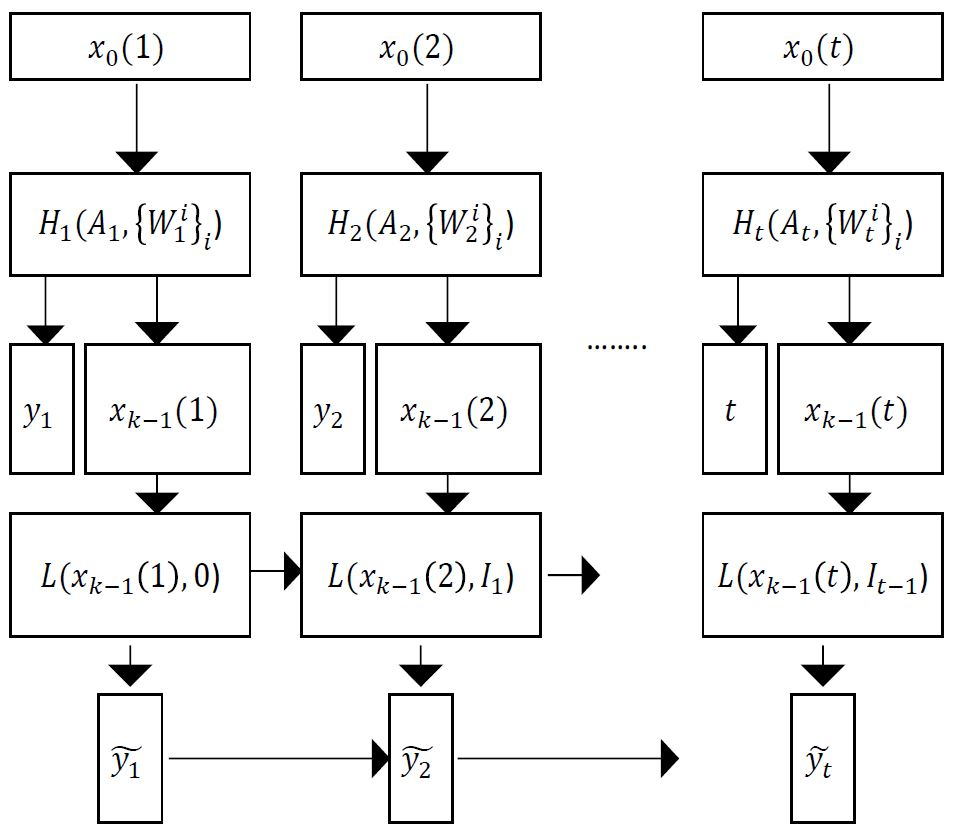
\includegraphics[width=\textwidth]{model}
    \centering
    \caption{\textit{Model description. The observations are input for all the nodes in the network for every TP $x_{0}(t)$ and a class for each node in each TP $z_{t}$. $x_{0}(t)$ is the input to a GCN $H_{t}$ that is based on the network in the TP $A_{t}$. We extract from the GCN the output values $y_{t}$ and the one before last layer $x_{k-1}(t)$. This layer is fed to an LSTM L which passed internal states and output to the following TP and produced a classification for each node in each time point $\tilde{y}_{t}$. In the first model, only the GCN was used and $y_{t}$ was compared to $z_{t}$. In the second model, the same analysis was performed, but the weights were shared among the $H_{t}$. In the following models, weights were still shared, but the comparison was between $\tilde{y}_{t}$ and $z_{t}$, The only difference between the third and fourth models is in the training. In the third model $H$ and $L$ were trained separately, and in the forth they were trained simultaneously.}}
    \label{fig:model}
\end{figure}
\section{Comparison of performances}
\subsection{Types of input}
When testing a topological input, we followed the Network Attribute Vector (NAV) approach of \cite{rosen2016topological,naaman2019edge}. In short, this approach presumes that the graph topological features (e.g. degree, clustering coefficient, centrality...) are correlated with the class of the node. As such these features can be used to predict the class of the node. We here deviate from this approach, by using the features as the input to a GCN, and letting the GCN combine these features with the adjacency matrix itself. For the NAV, we used the following topological features of each node: Attractor basin hierarchy \cite{muchnik2007self}, Flow measure \cite{rosen2014directionality} Average neighbor degree, Betweenness centrality, The first two moments of the distance distribution of each node to all other nodes, Closeness centrality, Eccentricity , Fiedler vector, K Core, Load centrality, Page Rank, and the frequency of small scale motifs surrounding each node, as proposed by Itzchack et al \cite{itzhack2007optimal}.
\\An alternative input is just using the trainning set node classification as an inputs. Formally, we count for each node the number of neighbors and second neighbors in the training set belonging to a class, leasding to a vector with twice the number of classes elements. We then tested each one of these inputs with or without the node information as inputs for different traning set fractions. We have thus tested the following 4 possible inputs:
\begin{enumerate}[A)]
\item   Topological features with inner content
\item   Topological features without inner content
\item   Neighbors data with inner content
\item   Neighbors data without inner content
\end{enumerate}
All the models outperform the results of JingFang et al (Figure \ref{fig:auc_inp_type}). The reuslts vary over the years, but the best results are for the combination of topology with external information, followed by the neighbors with internal information, followed by only the neighbor data, with a limited difference between the models, suggesting that the neighbor and topological infromation contain almost as much data as the detailed information in the balance sheets of the companies.

\begin{figure}[h!]
    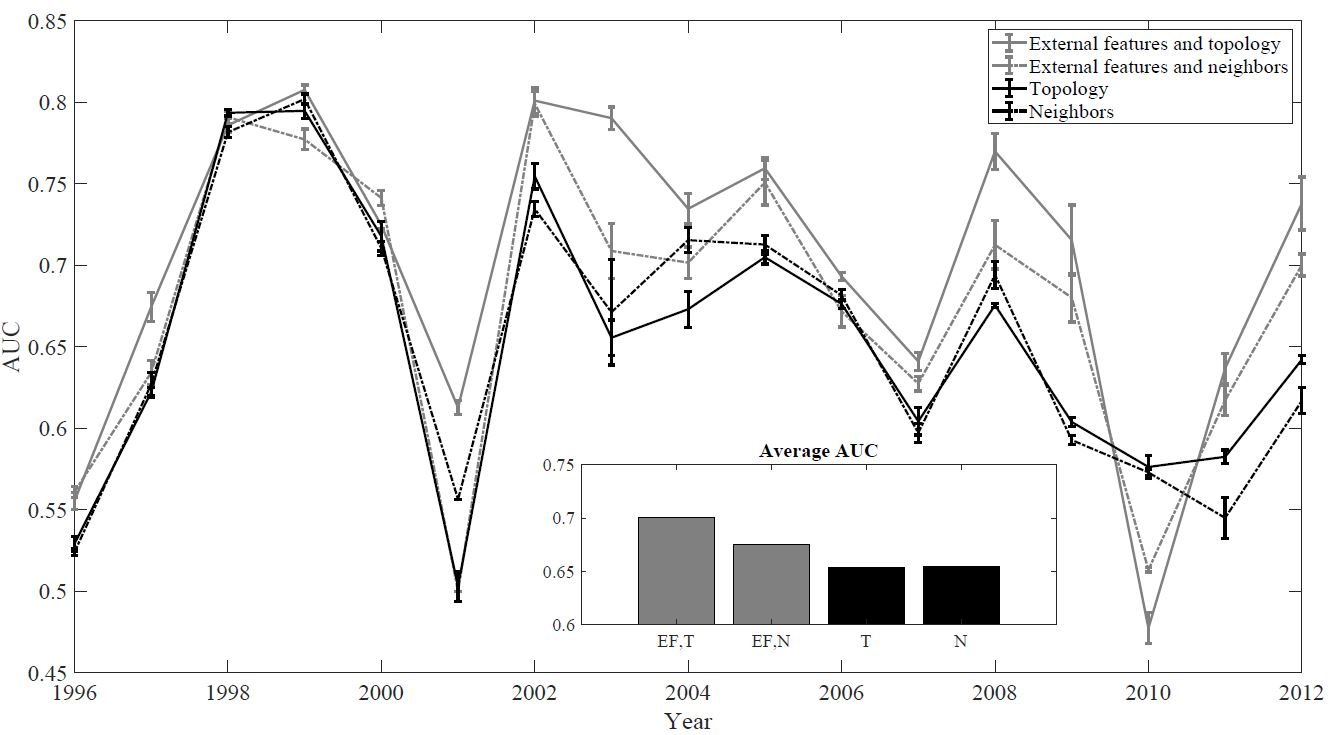
\includegraphics[width=\textwidth]{auc_inp_type}
    \centering
    \caption{\textit{Test AUC of the 4 types of input over the years and average (inset) for the first model. The gray lines use a combination of internal and topological information. The black lines use only topology. All models have a good accuracy in regular year (taking into account the complexity of predicting bankruptcy), but fail following crises (2000 and 2008). One can further notice that the models using the network topology and external information as input outperforms the others.}}
    \label{fig:auc_inp_type}
\end{figure}

\subsection{GCN-LSTM configration}
To test the effect of combining the GCN and LSTM we compared the different models above (Figure \ref{fig:auc_models_a}\ref{fig:auc_models_b}). The different models were trained either with or without internal information. Three interesting results emerge from the comparison. First, the precision varied significantly over the different years, and it drops following large scale crises to a random level (e.g. following the 2000 and 2008 crises). This may be the result of the large number of collapses that are not directly related to the regular market dynamics or the product portfolio. The second interesting result is that the combination with the RNN improves the performance, but the combined training of the GCN and the LSTM has a limited (yet significant) contribution to the accuracy. Moreover, the combined model is very sensitive to the initial conditions and often the loss does not converge to a low enough value. To resolve that, in the GCN-LSTM combined model, we performed multiple random initiations of the weights for a given training/test division. We then choose their realization with the best loss on the train. Finally, one can clearly see the effect of the LSTM in the crisis years, where the experience from a single year before is not enough to predict the collapse of companies, but the dynamic model manages to produce a better prediction. We have tested the same model for different types of input (as in the previous section) and different classifications with a similar ordering of the models (yet lower accuracies).
\\To further test the performance of the combined LSTM-GCN, we studied another network., where no external information was available. We again tested the 4 models using the topology as an input, and again the order of model performance is similar, with the GCN-LSTM drastically outperforming the GCN (Figure \ref{fig:auc_models_a}\ref{fig:auc_models_b}).
% \subsection{Combined model}
% HERE PLEASE CHECK A MODEL WHERE YOU DECIDE BASED ON THE TRAIN AUC WHETHER TO USE THE FULL MODEL OR WHETHER TO USE A SINGLE YEAR MODEL

\iffalse
\subsection{Types of input}
When testing a topological input, we followed the Network Attribute Vector (NAV) approach of
[24, 25]. In short, this approach presumes that the graph topological features (e.g. degree, clustering
coefficient, centrality...) are correlated with the class of the node. As such these features can be
used to predict the class of the node. We here deviate from this approach, by using the features as
the input to a GCN, and letting the GCN combine these features with the adjacency matrix itself.
For the NAV, we used the following topological features of each node: Attractor basin hierarchy
[26], Flow measure [27] Average neighbor degree, Betweenness centrality, The first two moments of
the distance distribution of each node to all other nodes, Closeness centrality, Eccentricity , Fiedler
vector, K Core, Load centrality, Page Rank, and the frequency of small scale motifs surrounding each
node, as proposed by Itzchack et al [28].
An alternative input is just using the training set node classification as an inputs. Formally, we count
for each node the number of neighbors and second neighbors in the training set belonging to a class,
leasding to a vector with twice the number of classes elements. We then tested each one of these
inputs with or without the node information as inputs for different training set fractions. We have thus
tested the following 4 possible inputs: A) Topological features with inner content, B) Topological
features without inner content, C) Neighbors data with inner content, and D) Neighbors data without
inner content. All the models outperform the results of JingFang et al (Figure 2). The reuslts vary
over the years, but the best results are for the combination of topology with external information,
followed by the neighbors with internal information, followed by only the neighbor data, with a
limited difference between the models, suggesting that the neighbor and topological infromation
contain almost as much data as the detailed information in the balance sheets of the companies.

When testing a topological input, we followed the Network Attribute Vector approach of (REF) and used the following topological features of each node: Attractor basin (REF),  Average neighbor degree, Betweenness centrality,  The first two moments of the distance distribution of each node to all other nodes,  Closeness centrality (REF), Eccentricity (REF), Fiedler vector (REF),  Flow measure (REF),  K Core (REF), Load centrality (REF), Page Rank (REF), and the frequency of small scale motifs surrounding each node (REF).
For stage 1 I ran 4 input scenarios:
•	Combined topological features with inner content
•	Combined topological features without inner content
•	Neighbors topological data with inner content
•	Neighbors topological data without inner content
As observed before, the best results came from the combination of topological features (all, including the neighbors, excluding motif4), with the inner data.
If we exclude the inner data, the neighbor's input achieved better than the combination of neighbors with topological features.
\fi

\section{Summary}
We have here shown that the future of companies can be predicted from their interaction networks, even in the absence of any other financial information. Previous works have shown that the topological information of this network combined with label propagation can be used to predict the future success or collapse of a network. We have shown that using GCN outperforms existing methods, as has been shown in many other graph machine learning domains \cite{kipf2016semi}. In the presence of multiple graphs, a single GCN is slightly better than a GCN for each graph, probably since the relation between the graph and the companies' success changes only slowly over time. However, when the same combined network is solved using an LSTM GCN, the performance is significantly increased, suggesting that while the dynamics of companies may change slowly, capturing the dynamics of the change allows the information from previous years to significantly improve on the accuracy of future years, especially following crises. The current formalism can be extended to any multi-network classification tasks, where the networks and tags change slowly enough.

\begin{figure}[h!]
    \begin{center}
         \subfigure[company network]{\label{fig:auc_models_a}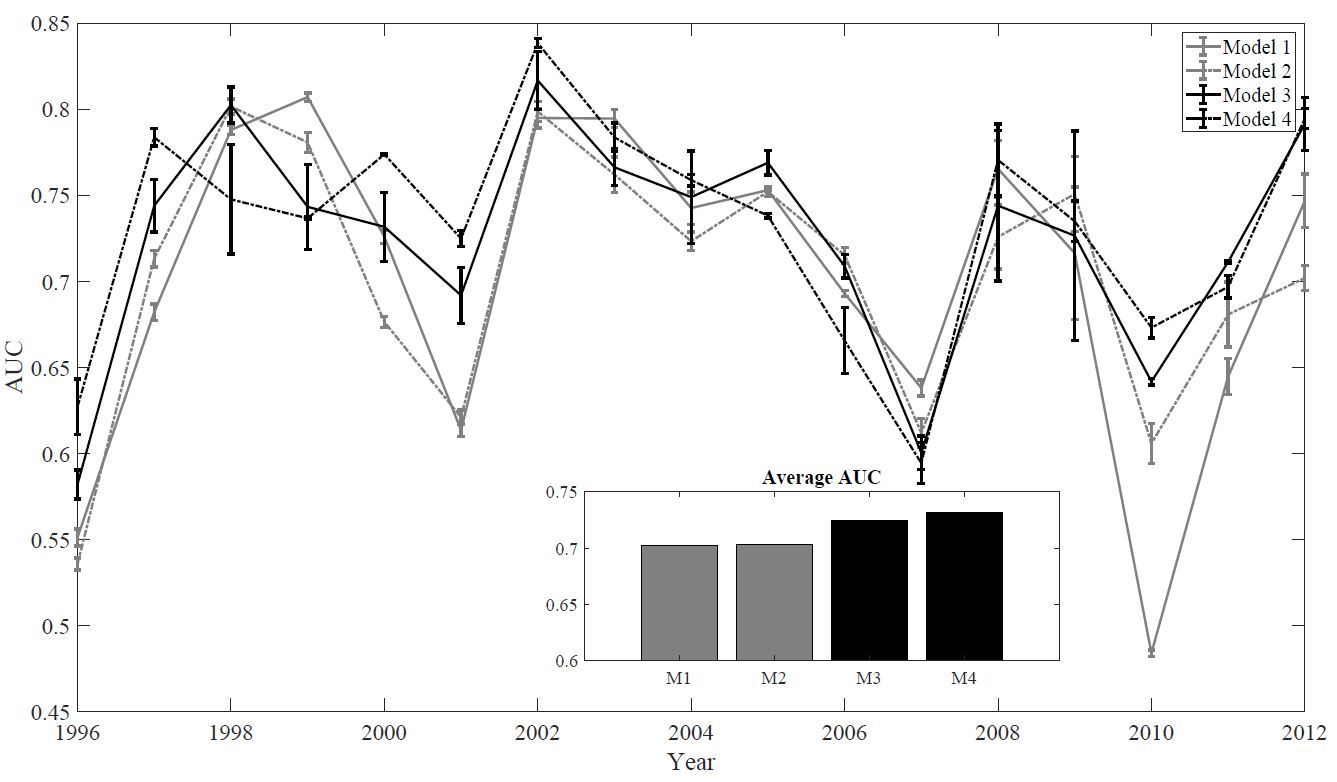
\includegraphics[width=\textwidth]{auc_models_a}}
         \subfigure[blog network]{\label{fig:auc_models_b}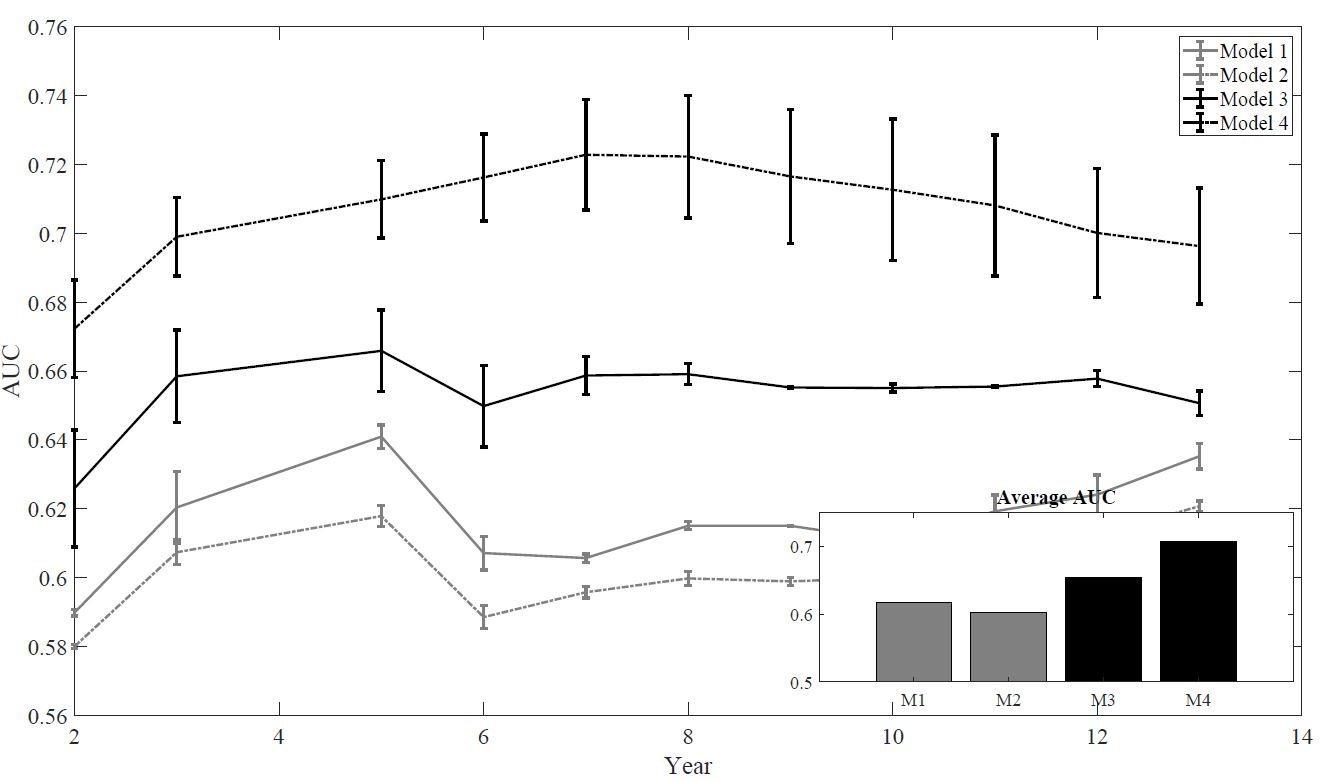
\includegraphics[width=\textwidth]{auc_models_b}}
    \end{center}
    \caption{\textit{Test AUC of the 4 models over the years and average (inset). We have here used only the best input type in the first model for consistency. The results with other input types all show the same ordering, but with lower accuracy.}}
    \label{fig:auc_models}
\end{figure}


\pagebreak
\bibliography{other/general}
% \input{parts/appendix}

\end{document}
